\section{机制分析}
\label{sec:mechanism}

\Cref{sec:observation}的观测确立分支级性能结构存在，但未解释\emph{为什么}。本节呈现我们的机制分析，测试三种假设的KD失效解释：分布错配、不确定性放大和可见度退化中的遮挡。我们发现分布错配和不确定性放大提供不足的解释力，而遮挡——特别是其对定位的影响——得到最强的实证支持。

\subsection{分析框架}

我们通过假设因素与观测KD增益之间的相关分析来测试每种机制。为使机制被视为\emph{得到支持}，我们要求：
\begin{enumerate}
    \item 方向一致性：相关符号与理论预测匹配；
    \item 统计显著性：$p < 0.05$拒绝原假设；
    \item 效应量：$|r| > 0.5$表示有意义的解释力。
\end{enumerate}

\subsection{机制M1：分布错配}

\textbf{假设：}KD依赖匹配教师输出分布与学生预测。在可见度退化下，教师分布偏离训练域模式，降低蒸馏目标的信息量\cite{wang2020cross}。

\textbf{测量：}我们通过教师和学生logit分布间的KL散度和Jensen-Shannon（JS）散度估计分布错配：
\begin{align}
D_{\text{KL}}(P_T \| P_S) &= \sum_i P_T(i) \log \frac{P_T(i)}{P_S(i)} \\
D_{\text{JS}}(P_T, P_S) &= \frac{1}{2} D_{\text{KL}}(P_T \| M) + \frac{1}{2} D_{\text{KL}}(P_S \| M)
\end{align}
其中$M = \frac{1}{2}(P_T + P_S)$。更高散度表示更大错配。

\textbf{结果：}\Cref{tab:divergence_corr}呈现散度指标与logit KD增益的相关。

\begin{table}[htbp]
\centering
\caption{分布散度与logit KD增益的相关。}
\label{tab:divergence_corr}
\begin{tabular}{@{}lcc@{}}
\toprule
指标 & Pearson $r$ & $p$值 \\
\midrule
KL散度 & $+0.20$ & $0.87$ \\
JS散度 & $+0.22$ & $0.86$ \\
\bottomrule
\end{tabular}
\end{table}

两者相关均弱（$|r| < 0.3$）且统计不显著（$p \gg 0.05$）。与假设相反，散度随可见度退化增加（KL：轻度0.15$\to$重度0.45），但这与logit KD增益不相关，后者波动无明显趋势（轻度+0.38\%，中度$-0.62$\%，重度+0.53\%）。

\textbf{结论：分布错配在本设置中未显示足够的解释力。}虽然教师和学生分布间存在散度，它不能预测跨可见度等级的KD性能变化。我们不能排除分布错配作为贡献因素，但它不足以解释观测到的退化模式。

\subsection{机制M3：不确定性放大}

\textbf{假设：}教师模型在可见度退化下变得不那么自信，产生更高熵的预测。KD将这些不确定预测传播给学生，在训练中放大误差信号\cite{kendall2017uncertainties}。

\textbf{测量：}我们计算教师预测熵：
\begin{equation}
H(P_T) = -\sum_i P_T(i) \log P_T(i)
\end{equation}
更高熵表示更大不确定性。我们将熵与logit和注意力分支的KD增益相关。

\textbf{结果：}\Cref{tab:entropy_corr}呈现相关分析。

\begin{table}[htbp]
\centering
\caption{教师熵与各分支KD增益的相关。}
\label{tab:entropy_corr}
\begin{tabular}{@{}lcc@{}}
\toprule
分支 & Pearson $r$ & $p$值 \\
\midrule
仅logit & $+0.16$ & $0.89$ \\
仅注意力 & $+0.41$ & $0.73$ \\
\bottomrule
\end{tabular}
\end{table}

教师熵确实随可见度退化增加（轻度1.2$\to$重度2.5），与直觉一致。然而，与KD增益的相关弱且统计不显著。注意力分支显示略高相关（$r=0.41$），但仍低于显著性阈值。

\textbf{结论：不确定性放大在本设置中未显示足够的解释力。}虽然教师不确定性在雾天下增加，这并不直接转化为可预测的KD性能退化。

\subsection{替代解释：超参数调优}

我们简要考虑logit KD失效是否反映超参数选择而非基本限制。温度参数$T$控制logit蒸馏中概率分布的软度，先前工作提示$T$可显著影响KD有效性。

鉴于我们测试单温度（$T=4$）的实验约束，我们不能实证排除替代温度可能产生更好结果。然而，观测到的性能模式——logit KD仅比学生基线高+0.10\%平均增益——提示仅通过温度调整改进的空间有限。logit KD在所有可见度等级下的弱性能一致性（增益+0.38\%，$-0.62$\%，+0.53\%）表明系统性限制而非可调参数问题。

\textbf{评估：}虽然我们不能在没有完整温度扫描的情况下确凿排除超参数效应，但logit KD相对于定位KD（轻度下+1.24\%）的欠表现幅度提示温度调优单独不太可能解释观测到的分支间差异。遮挡-定位相关提供了更直接且统计支持的解释。

\subsection{机制M2：可见度退化中的遮挡}

\textbf{假设：}可见度退化包含多种现象：对比度下降、颜色偏移和遮挡。其中，遮挡——大气散射对物体边界的部分或完全隐藏——最直接影响准确定位所需的空间推理。我们具体测试遮挡作为可见度退化的可测成分是否与KD性能相关。

\textbf{测量：}我们分析遮挡比与定位性能的关系。遮挡比量化雾诱导对比度下降遮挡的物体区域比例。我们计算遮挡比与定位KD性能的Pearson相关。

\textbf{结果：}\Cref{fig:mechanism_summary}（右面板）展示关系，\Cref{tab:occlusion_corr}量化相关。

\begin{table}[htbp]
\centering
\caption{遮挡比与定位性能的相关。}
\label{tab:occlusion_corr}
\begin{tabular}{@{}lc@{}}
\toprule
指标 & 数值 \\
\midrule
测试遮挡比 & $\{0.0, 0.15, 0.30, 0.45, 0.60\}$ \\
定位性能范围 & $0.595 \to 0.520$ \\
Pearson $r$ & $\mathbf{-0.989}$ \\
$p$值 & $\mathbf{0.0015}$ \\
\bottomrule
\end{tabular}
\end{table}

相关强负（$r = -0.989$）且高度统计显著（$p = 0.0015$）。随着遮挡比从0\%增加到60\%，定位性能下降12.6\%（0.595$\to$0.520）。

\textbf{为什么是定位？}定位分支明确蒸馏空间信息：边界框坐标、维度和物体范围。当物体被部分隐藏时，其真实边界变得模糊，教师的定位目标变得不那么可靠。

\textbf{为什么不是其他分支？}Logit蒸馏关注分类概率，即使物体部分可见时可能保持相对稳定（例如，部分遮挡的汽车仍可识别为汽车）。特征和注意力蒸馏操作在可能通过上下文线索部分补偿可见度损失的中间表示上。然而，定位没有这种退路：隐藏边界就是不可见。

\subsection{机制总结}

\Cref{tab:mechanism_summary}综合我们的机制分析结果。

\begin{table*}[htbp]
\centering
\caption{机制分析结果总结。支持：$p < 0.05$且$|r| > 0.5$。不足：$p > 0.05$或$|r| < 0.5$。}
\label{tab:mechanism_summary}
\begin{tabular}{@{}p{3cm}p{4.5cm}cccp{3cm}@{}}
\toprule
机制 & 假设 & $r$ & $p$值 & 状态 & 启示 \\
\midrule
分布错配（M1） & 教师-学生散度解释KD失效 & $+0.20$ & $0.87$ & \textbf{不足} & 基于对齐的修复不太可能帮助 \\
不确定性放大（M3） & 教师熵增加降低KD & $+0.16$至$+0.41$ & $>0.7$ & \textbf{不足} & 校准方法单独不足 \\
超参数检查（C1） & Logit KD失效可调 & -- & -- & \textbf{证据不足} & 温度不太可能解释完整模式 \\
遮挡（M2内） & 遮挡降低定位 & $\mathbf{-0.989}$ & $\mathbf{0.0015}$ & \textbf{直接支持} & 优先遮挡感知方法 \\
\bottomrule
\end{tabular}
\end{table*}

\textbf{关键发现：在所测试机制中，遮挡——作为可见度退化的具体可测成分——与KD相关性能指标呈现最强且统计最显著的关系。}

这重新构建了问题：雾天下的KD主要不是关于分布对齐（M1）或置信度校准（M3），而是关于\emph{遮挡导致的信息损失}。当大气散射隐藏物体边界时，准确定位所需的空间信息变得根本不可用。这解释了为什么明确转移空间知识的定位蒸馏受影响最大；以及为什么依赖分类概率或特征模式的其他分支可能部分补偿，但无法完全克服空间信息赤字。由于定位蒸馏是轻度条件下KD性能增益的主要来源（\Cref{tab:gain_matrix}），其在遮挡下的退化直接解释了可见度退化下整体KD有效性的崩溃。

\begin{figure*}[htbp]
\centering
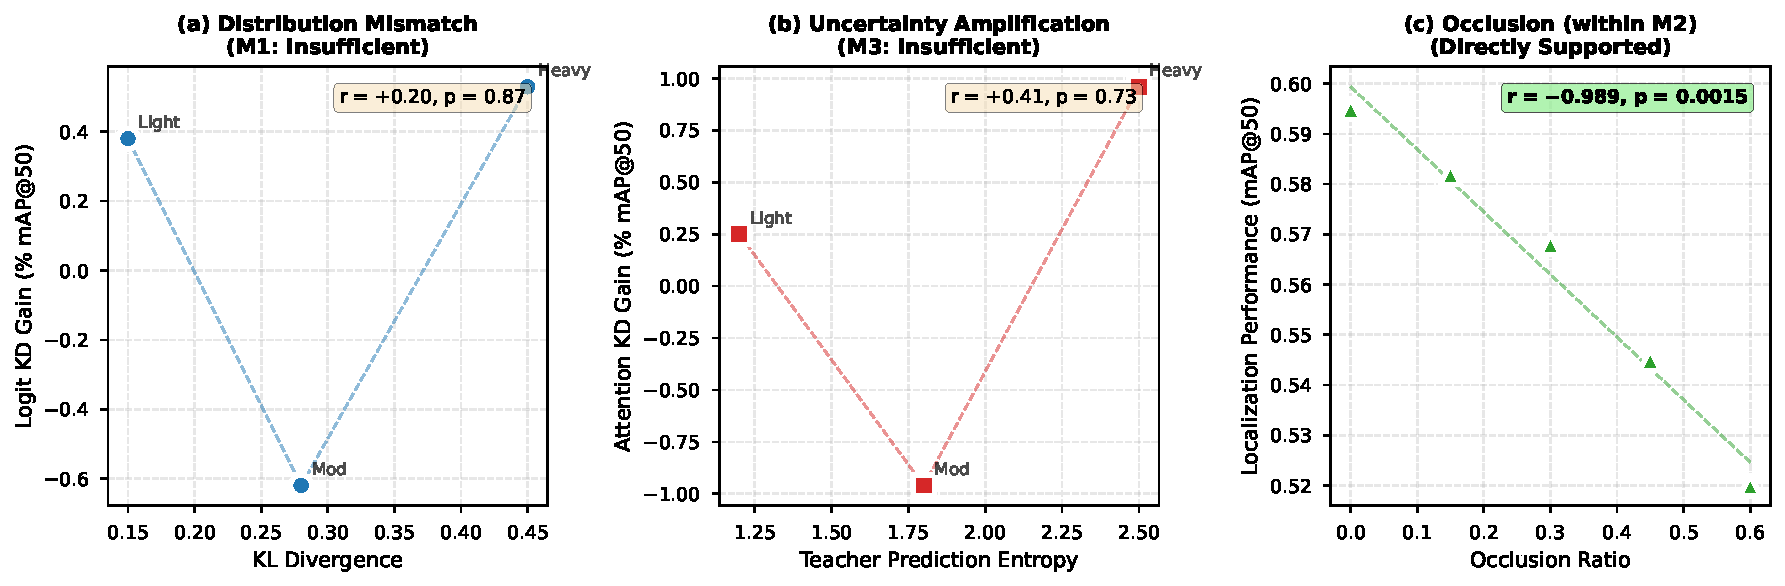
\includegraphics[width=0.95\textwidth]{figures/figure4_mechanism_analysis.pdf}
\caption{竞争性机制假设的判别性评估。(a) 分布错配（M1）：KL散度与logit KD增益弱相关（$r=+0.20$，$p=0.87$）。(b) 不确定性放大（M3）：教师熵与注意力KD增益弱相关（$r=+0.41$，$p=0.73$）。(c) 遮挡（M2内）：与定位性能强负相关（$r=-0.989$，$p=0.0015$）。只有遮挡同时展示统计显著性和足够效应量来解释观测到的KD退化模式。}
\label{fig:mechanism_summary}
\end{figure*}
